% Allow relative paths in included subfiles that are compiled separately
% See https://tex.stackexchange.com/questions/153312/
\providecommand{\main}{..}
\documentclass[\main/thesis.tex]{subfiles}

\begin{document}

\chapter{Introduction}
\section{What is our goal?}
Our goal is to create a new, virtual source of novel drum sounds. A common approach to creation of drum tracks for digital music is to combine short recordings of real-life drums and other percussive elements in order to create a new drum-kit. This approach frees artists from the need to obtain and store real life instruments while enabling endless combinatorial possibilities. However, by relying on recordings of \textit{real life} drum sounds, we are still limited by what drums exist in the real world and whether or not we have access to clean, one-shot\footnote{A single hit on the drum that captures its capabilities} recordings of these drums.

To find new sources of novel drum sounds, we can conceptualize utilizing digital sound synthesis in various ways. An ideal scenario would be a graphical, 3D simulation of virtual drums; Where we could modulate the thickness, dimensions and material of the frame, the drum skin, the type of impact, etc. before rendering the sound of the simulation. Unfortunately, such 3D systems are not yet practical \cite{langlois2016toward}. State of the art generative networks utilized in works such as \cite{ramires2019timbfeat,aouameur2019neural} are another promising avenue; However, as discussed further in \ref{related} we prefer to work towards more efficient methods that utilize simple, tried and true methods of digital sound synthesis in tandem with machine learning techniques to rapidly generate new sounds. Another desirable (by us) by-product of this approach is that the sounds generated may sound extremely in-organic, yet perfectly usable by more experimental artists.

\section{How Can A Computer Make Sounds?}
Your computer can make a wide variety of sounds in wide variety of ways. You can use it to record real life audio and play it back. You can hit its various parts with a drumstick. You can also program it to make noise at a software level. 

Sounds are transmitted via waveforms. Your computer can emulate the physical characteristics of basic waveforms by evaluating the output of periodic functions such as sines and cosines. Evaluation of basic periodic functions is the simplest form of software audio generation \cite[chapter~5]{mitchell2009basicsynth}.

For example, think of the universally recognizable "dialing" sounds that communication networks use during typical phone calls. You can program your computer to make similar noises by feeding a range of equally spaced values between 0 and $2\pi$ to a sinusoidal function at a rate that's audible to human ears\footnote{Human audible range is approximately 30Hz to 15000KHz}. This generative system is called an \textit{oscillator} and its output is a waveform which can be sent to your computer's digital-to-analog conversion system to create an audible signal. The combination and modification of these pure tones are the building blocks of digital signal processing (DSP).
% make circle/wave graph from chapter 5 of mitchell
\begin{figure*}[h]
\centering
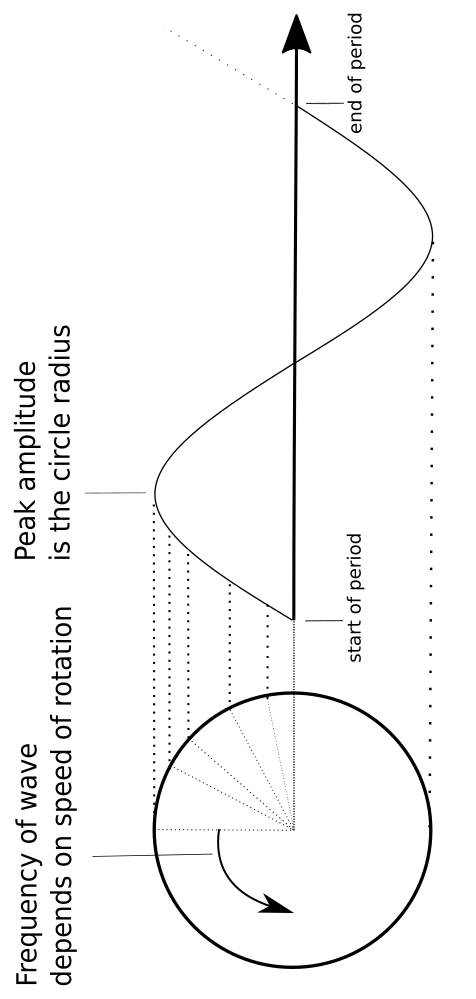
\includegraphics[width=0.45\linewidth,angle =-90 ]{images/periodic_function.png}
\caption{A computer can simulate waveforms by utilizing periodic functions. Digital waveforms are discrete approximations of analogue waves. }
\end{figure*}


 Most organic sounds are much more complex than the output of a single oscillator and their digital approximation requires a combination of multiple (perhaps thousands) of pure tones. However, with careful programming, DSP techniques can be used to replicate almost any sound, which is why they have powered commercial digital synthesizers for over half a century \cite{jenkins2019analog} and continue to remain a popular method of audio synthesis amongst artists. Another advantage to using DSP for sound generation is that the synthesizers we build using these functions are tractable: the output is determined by the input and reproducible. This makes the evaluation of a set of inputs (or parameters) to our synthesizers  simpler compared to the evaluation of synthesizers that utilize probabilistic models.
 
 %talk about vsts here

\section{How Can a Computer Categorize Sounds?}
Suppose a human is given a set of recordings of solo musical instruments being played by various skill levels and asked to categorize them however they please. There is a long list of features that the human could use: the length of audio recordings, the skill of the player, the timbre of the instrument (which is related to the type of instrument: wind, string, percussion etc.) the rhythm and so on. 

Computers can be programmed to extract the majority of these feature types for us. Particularly with shorter audio clips (such as the drum sounds we're interested in) where human subjectivity might play a smaller role in describing sounds and the categorization task becomes easier. 

In our work, we find simple features such as frequency content (high pitch vs low pitch), length, and envelope (change in loudness, how fast the sounds reaches its maximum loudness and fades away) to be powerful in categorization of drum sounds. Later on we will discuss our algorithms for extraction of these and other features in \ref{impl}. We will also discuss how these extracted features were used to train models that can automatically categorize new sounds. 

\section{What Is Our Methodology?}

Our attempt is centered around a generative pipeline of audio. The outputs of this pipeline are evaluated and the evaluation score is used to improve further improve the pipeline and separate undesired outputs from desired ones. We want random sounds to be created by a tractable source, we also want to evaluate these sounds so we can guide the random sound generator towards desired sounds. Instead of learning weights and parameters in an audio-generation neural network, we wish to generate, search, and tune synthesizers to produce percussion sounds. Following this idea, we found the proper implementation of 2 major components to be crucial:

\begin{itemize}
    \item \textit{Virtual Synthesizer}: A flexible, deter\-min\-istic, and tract\-able gener\-ator which can create audio. 
    \item \textit{Virtual Ear}: An ear that returns an evaluation of an audio sample; estimating the effectiveness of an audio sample's fulfillment of a producers requirements. The ear's evaluation guides the generation process towards a desired path, making it a crucial component of our pipeline. 
\end{itemize}
% AH: Optional. Can be removed or reduced later
Our components are designed with modularity and parallelizability in mind. This allows each component to be debugged, modified, and improved without requiring modifications in other components while additionally increasing the scalability and speed of experiments. 
Section \ref{impl} contains further discussion of the components as well as the code that glues the project together.

While the main focus of this project is the generation of novel percussive sounds, our methodology indicates promising results with regards to creation of new presets for any virtual synth without the need for a-priori knowledge of the functions or its parameters (i.e the effect of parameter modulation on the sonic output). We also demonstrate the viability of a virtual synthesizers based on Digital Signal Processing (DSP) methods for fast, unsupervised creation of novel audio, discussed in more detail in section \ref{related}. 


\section{Data And Project Replication}
\label{data}
Our data is a large set of drum samples aggregated from personal libraries, free drum kits from the sample-swap project \footnote{https://sampleswap.org/} which we further processed to suit our categories, and a large set of drum sounds aggregated from royalty free sources such as musicradar \footnote{https://www.musicradar.com/}. We have made our dataset of free-drum sounds available for download. The scripts used to download and process royalty free samples will also be made available. Further information about downloading our dataset can be found on this project's github page. 

Our drum categories are claps, hats, kicks, rims/other, shakers, snares and toms. Other categories are chopped guitars, chopped pianos and n-stack-synths (random noise generated by the virtual synth with stack size of n, see \ref{vs}), utilized for learning percussive vs non-percussive sounds. Stack sizes refers to how many synth functions are connected together in a synthesizer.
Some notes about our dataset:


\begin{itemize}
\item Of the 6000 drum-sounds utilized in our work, the kick, snare and hat categories have the largest share at around 20\% each, while the shaker and rim (other) categories have the smallest at 5\% combined. Due to this we only focused on learning from kicks, snares, toms, claps and hats for Phase 1 of training (along with non-percussive groups of sound) \ref{sec:ear}.

\item For Phase 2 of training we only focused on categorizing snares, claps, kicks, hats and other (percussive sounds such as shakers, rims and unusual percussions that we couldn't categorize were grouped into this category). Non-percussive datasets were not used for this phase. 
\item In order to offset bias from data imbalance during training of our models, the categorical cross entropy loss was weighted by the group sizes. 
\item For any given model, 80\% of our data is used for training and 20\% is used for testing. 

\item We limit the size of the n-stack-synths category to 50\% of the total size of our drum dataset. This is done in order to measure whether the features extracted can address the "Open Set Recognition" problem, which will be discussed further in Section \ref{sec:ear}.
\end{itemize}

\section{Restating the the Goal}
We want to leverage AI technologies, such as heuristic search and random search, to produce new drum samples, by finding synthesizers and their appropriate configurations that can produce various kinds of drum samples. Effectively we will combine machine listening and code generation of synthesizers to find drum samples.

Our work is motivated by the idea of finding new, convenient methods for the expansion of a music producer's library of sounds. Primarily with generation of novel, one-shot audio samples but also with automated search and creation of presets for virtual synthesizers. Using the generation of short, percussive audio samples as a starting point, this project is a proof of concept for a promising avenue towards our motivational goal.

\end{document}